\documentclass{article}
\usepackage{xeCJK}
  \xeCJKsetup{%
    %PunctStyle=kaiming,
    CJKspace=true,% % true이면 띄어쓰기 사용. 중국어, 일어는 필요 없을수도
    % CJKmath=true,%  % true면 math environment 안에서 CJK 글자 사용
    CJKecglue={}%   % Western과 CJK 사이의 공백 지정: {}로 간격을 없앰
  }
%\usepackage[UTF8]{ctex}

% \setmainfont{Noto Serif}
%\setCJKmainfont{gulim.ttf}
%\setCJKsansfont{gulim.ttf}
%\setCJKmonofont{gulim.ttf}
%\setCJKmainfont{}

% below specific to Chinese version
\setCJKmainfont{Noto Serif CJK SC}
\setCJKsansfont{Noto Serif CJK SC}
\setCJKmonofont{Noto Serif CJK SC}
\usepackage{indentfirst}
\setlength{\parindent}{2em}

% Language setting
% Replace `english' with e.g. `spanish' to change the document language
\usepackage[english]{babel}
\usepackage{listings}
\usepackage{minted}
% Remove this draft watermark for the final version
% \usepackage{draftwatermark}

% Set page size and margins
% Replace `letterpaper' with `a4paper' for UK/EU standard size
\usepackage[letterpaper,top=2cm,bottom=2cm,left=3cm,right=3cm,marginparwidth=1.75cm]{geometry}

% Useful packages
\usepackage{amsmath}
\usepackage{comment}
\usepackage{graphicx}
\usepackage{IEEEtrantools}
\usepackage[hyphens]{url}
\usepackage[colorlinks=true, allcolors=blue]{hyperref}

\usepackage{setspace}
  \onehalfspacing
  % \setstretch{1.25} % custom spacing

\title{Aptos 区块链:安全、可扩展和可升级的 Web3 基础设施}
\author{}
\date{2022 年 8 月 11 日\\v1.0}

\begin{document}
\maketitle

\begin{comment}

Goals: 
* Introduce the problems we are solving in web3
* Introduce our approach and our solutions to reliability, scalability, and upgradeability while preserving decentralization
* Differentiate our approach from others in the web3 space
Provide the appropriate level of detail - especially for future work (more detail on areas we have more information and more directional on areas we still need to do research/eng)

Terminology:
* Nodes - full nodes or validators
* Uppercase Internet
* Aptos blockchain - do not use Aptos protocol
* up-to-date, not up to date
* Ledger state and ledger history
* Avoid the word database in the context of blockchain
* trade-offs not tradeoff
* upgradeable, not upgradable
* web3, not Web3 unless at the beginning of a sentence.
* dApp is out-of-date, just applications are fine.
* high throughput not high-throughput

Formatting:
* After end{itemize} or end{enumerate}, start the next sentence immediately so the indent is far to the left instead of indented

\end{comment}

    % Someone needs to convert 'abstract' and 'figurename' to chinese below
\renewcommand{\abstractname}{摘要}
\renewcommand{\figurename}{图}

\begin{abstract}
随着全新的互联网基础设施区块链的崛起,开发者正以飞快的速度部署着数以万计的去中心化应用程序。遗憾的是,由于稳定性差、成本高、低吞吐量及一些安全问题,区块链尚未被广泛应用。 为了能够在web3时代被广泛使用,区块链基础设施应该效仿云基础设施的特点,即为众多的去中心化应用提供可信,可扩展,经济高效且持续优化的平台。

为应对这些挑战,我们以可扩展、安全、可靠和可升级为核心设计原则推出\emph{Aptos 区块链}。 Aptos 区块链是在过去三年中由全球350多名开发人员开发的 \cite{aptos_core_github}。 它在共识算法、智能合约设计、系统安全、性能和去中心化方面提供了新的创新。 这些技术的结合将为把Web3带向更广泛的人群提供一个坚实的基础:
\footnote{法律免责声明:本白皮书及其内容不是出售任何代币的要约,也不是诱导购买任何代币的要约。 我们发布这份白皮书只是为了接受公众的反馈和意见。 本文件中的任何内容都不应被理解为对Aptos区块链或其代币 (若有) 将如何发展、利用或累积价值的保证或承诺。 Aptos仅概述了其目前的计划,这些计划可能会酌情改变,其成功与否将取决于其控制之外的许多因素。 这种未来的陈述必然涉及已知和未知的风险,这可能导致未来时期的实际表现和结果与我们在本白皮书中描述或暗示的有重大差异。 Aptos不承担更新其计划的义务。 不能保证白皮书中的任何陈述将被证明是准确的,因为实际结果和未来事件可能有很大的不同。 请不要过分依赖未来的声明。}
 
 \begin{itemize}
  \item 首先,Aptos 区块链原生集成并使用 \emph{Move 语言}来实现快速安全的交易执行 \cite{move_github}。 \emph{Move prover},一个用Move 语言开发的智能合约形式化验证工具,为合约常量和运行提供额外保障。 这种注重安全的做法,可以让开发人员能够更好地保护软件,以免受恶意实体的攻击。 
  \item 其次,Aptos 数据模型允许灵活的密钥管理和混合托管选项。 这与签名前的交易透明性和实用的轻客户端协议一起,共同提供了更安全、更值得信赖的用户体验。

  \item 第三,为了实现高吞吐量和低延迟,Aptos区块链在交易处理的关键阶段使用了流水线和模块化方法。 具体而言,交易分发、区块元数据排序、并行事务执行、批量存储和账本认证等操作会同时运行。 这种做法充分利用了所有可用的硬件资源,提升了硬件效率,并实现了高度并行处理。 

  \item 第四,与需要读写前获取被读写数据而破坏交易原子性的并行执行引擎不同,Aptos 区块链没有对开发者设置这种限制。它通过保证复杂的交易的原子性,为应用程序提供更高的吞吐量和更低的延迟,并简化了开发。

  \item 第五,Aptos模块化架构保证了客户端的灵活性,并针对频繁的升级进行优化。 此外,为了迅速部署新的技术创新和支持新的Web3使用案例,Aptos区块链提供了嵌入式的链上变化管理协议。

  \item 最后,Aptos区块链正在试验未来超越单个验证器性能的举措:其模块化设计和并行执行引擎支持验证者的内部分片,而同质状态分片(homogeneous state sharding)提供了水平吞吐量可扩展的潜力,而不会给节点运营商带来额外的复杂性。
\end{itemize}

\end{abstract}

\section{引言}

在 web2 时代,诸如通讯、社交媒体、金融、游戏、购物以及音视频流媒体等服务, 是由掌握了用户数据权限的中心化公司来提供(例如Google、Amazon、Apple和Meta)。 针对目标用例,这些公司利用具备特定应用的软件,来优化开发基础设施,并利用云端基础设施向用户部署这些应用程序。 云端基础设施可提供虚拟或物理基础设施服务的访问,例如虚拟机租用 (VMs)和在世界各地数据中心内运行的裸机硬件(例如AWS,Azure,和 Google Cloud)。 因此,建立能够扩大到数十亿用户的 web2 互联网服务从来没有像今天这样容易。 然而,web2要求用户明确信任中心化实体,这一要求愈发引起社会的担忧。

为了消除这种担忧,新的互联网时代已经开始:web3。 在 web3 版本的互联网中, 出现了区块链来提供去中心化、不可篡改的账本,让用户能够安全可靠地相互交流,而不需要信任控制中间人或中心化实体。 与 web2 互联网服务和应用程序依赖云基础设施类似,去中心化的应用程序可以使用区块链作为去中心化的基础设施层,从而触达全世界数十亿用户。

然而,尽管今天存在许多区块链,但是 web3 尚未得到广泛采纳~\cite{a16_state}。 虽然技术不断地推动着行业发展,但现有的区块链仍是不可靠的。昂贵的交易费用,低吞吐量,因安全问题资产经常遭受损失,并且无法支持实时响应。 与云端基础设施赋能 web2 服务,成功触达数十亿人群相比,区块链还并没有使得 web3 应用达到同样的高度。

\section{Aptos 愿景}

Aptos的愿景是提供一个能够为 web3 带来主流应用的区块链,并授权一个去中心化应用的生态系统来解决现实世界的用户痛点。 我们的使命是通过提供灵活和模块化的区块链架构,推动区块链可靠性、安全性和性能方面的新高度。 该架构应支持频繁升级,快速采用最新的技术,并能对新兴的用例提供一流支持。

我们设想建立社区管理运营的去中心化、安全和可扩展的网络。 当世界各地对基础设施的需求增长时,区块链的计算资源就会横向和纵向扩展以满足这些需求。 随着新的用例和技术进步的出现,网络应该在不干扰用户的情况下频繁地、无缝地升级。 让用户不再关注基础设施相关问题。 开发人员和用户将可以访问许多不同的密钥恢复、数据建模、智能合约标准、资源使用权衡、隐私和可组合性选项。 用户确信他们的资产是安全,可用,并且几乎可以成本费访问。 任何人都能够安全、容易地与全世界不受信任的各方进行不可篡改的交易。 区块链将像云基础设施一样无所不在。

为了实现这一愿景,必须在技术方面取得重大进展。 过去三年里,我们开发,升级和部署Diem区块链(Aptos区块链的前身) 的经验已经证明,网络可以在不中断客户端的情况下持续升级协议\cite{diem_blockchain}。 2020年初,Diem主网被部署到拥有多个钱包供应商的十几个节点上。 在之后一年,我们团队进行了共识协议和核心框架两次重大的升级。 两次升级都在用户不停机的情况下顺利完成。 在 Aptos 区块链中,我们对技术栈进行了一系列彻底的改进,同时还受到 Diem 区块链的启发,将安全、透明、以及可频繁的升级作为核心功能。 我们特别强调新的交易处理方法(如第 \ref{sec:pipelining_batching} 节所述) 以及去中心化和网络治理的新方法。

随着Aptos区块链的不断改善和发展,, 我们将不断更新协议和设计,届时发布最新版的白皮书。 在下文中,我们描述了 Aptos 区块链的现状以及今后的计划。

\begin{figure}
\centering
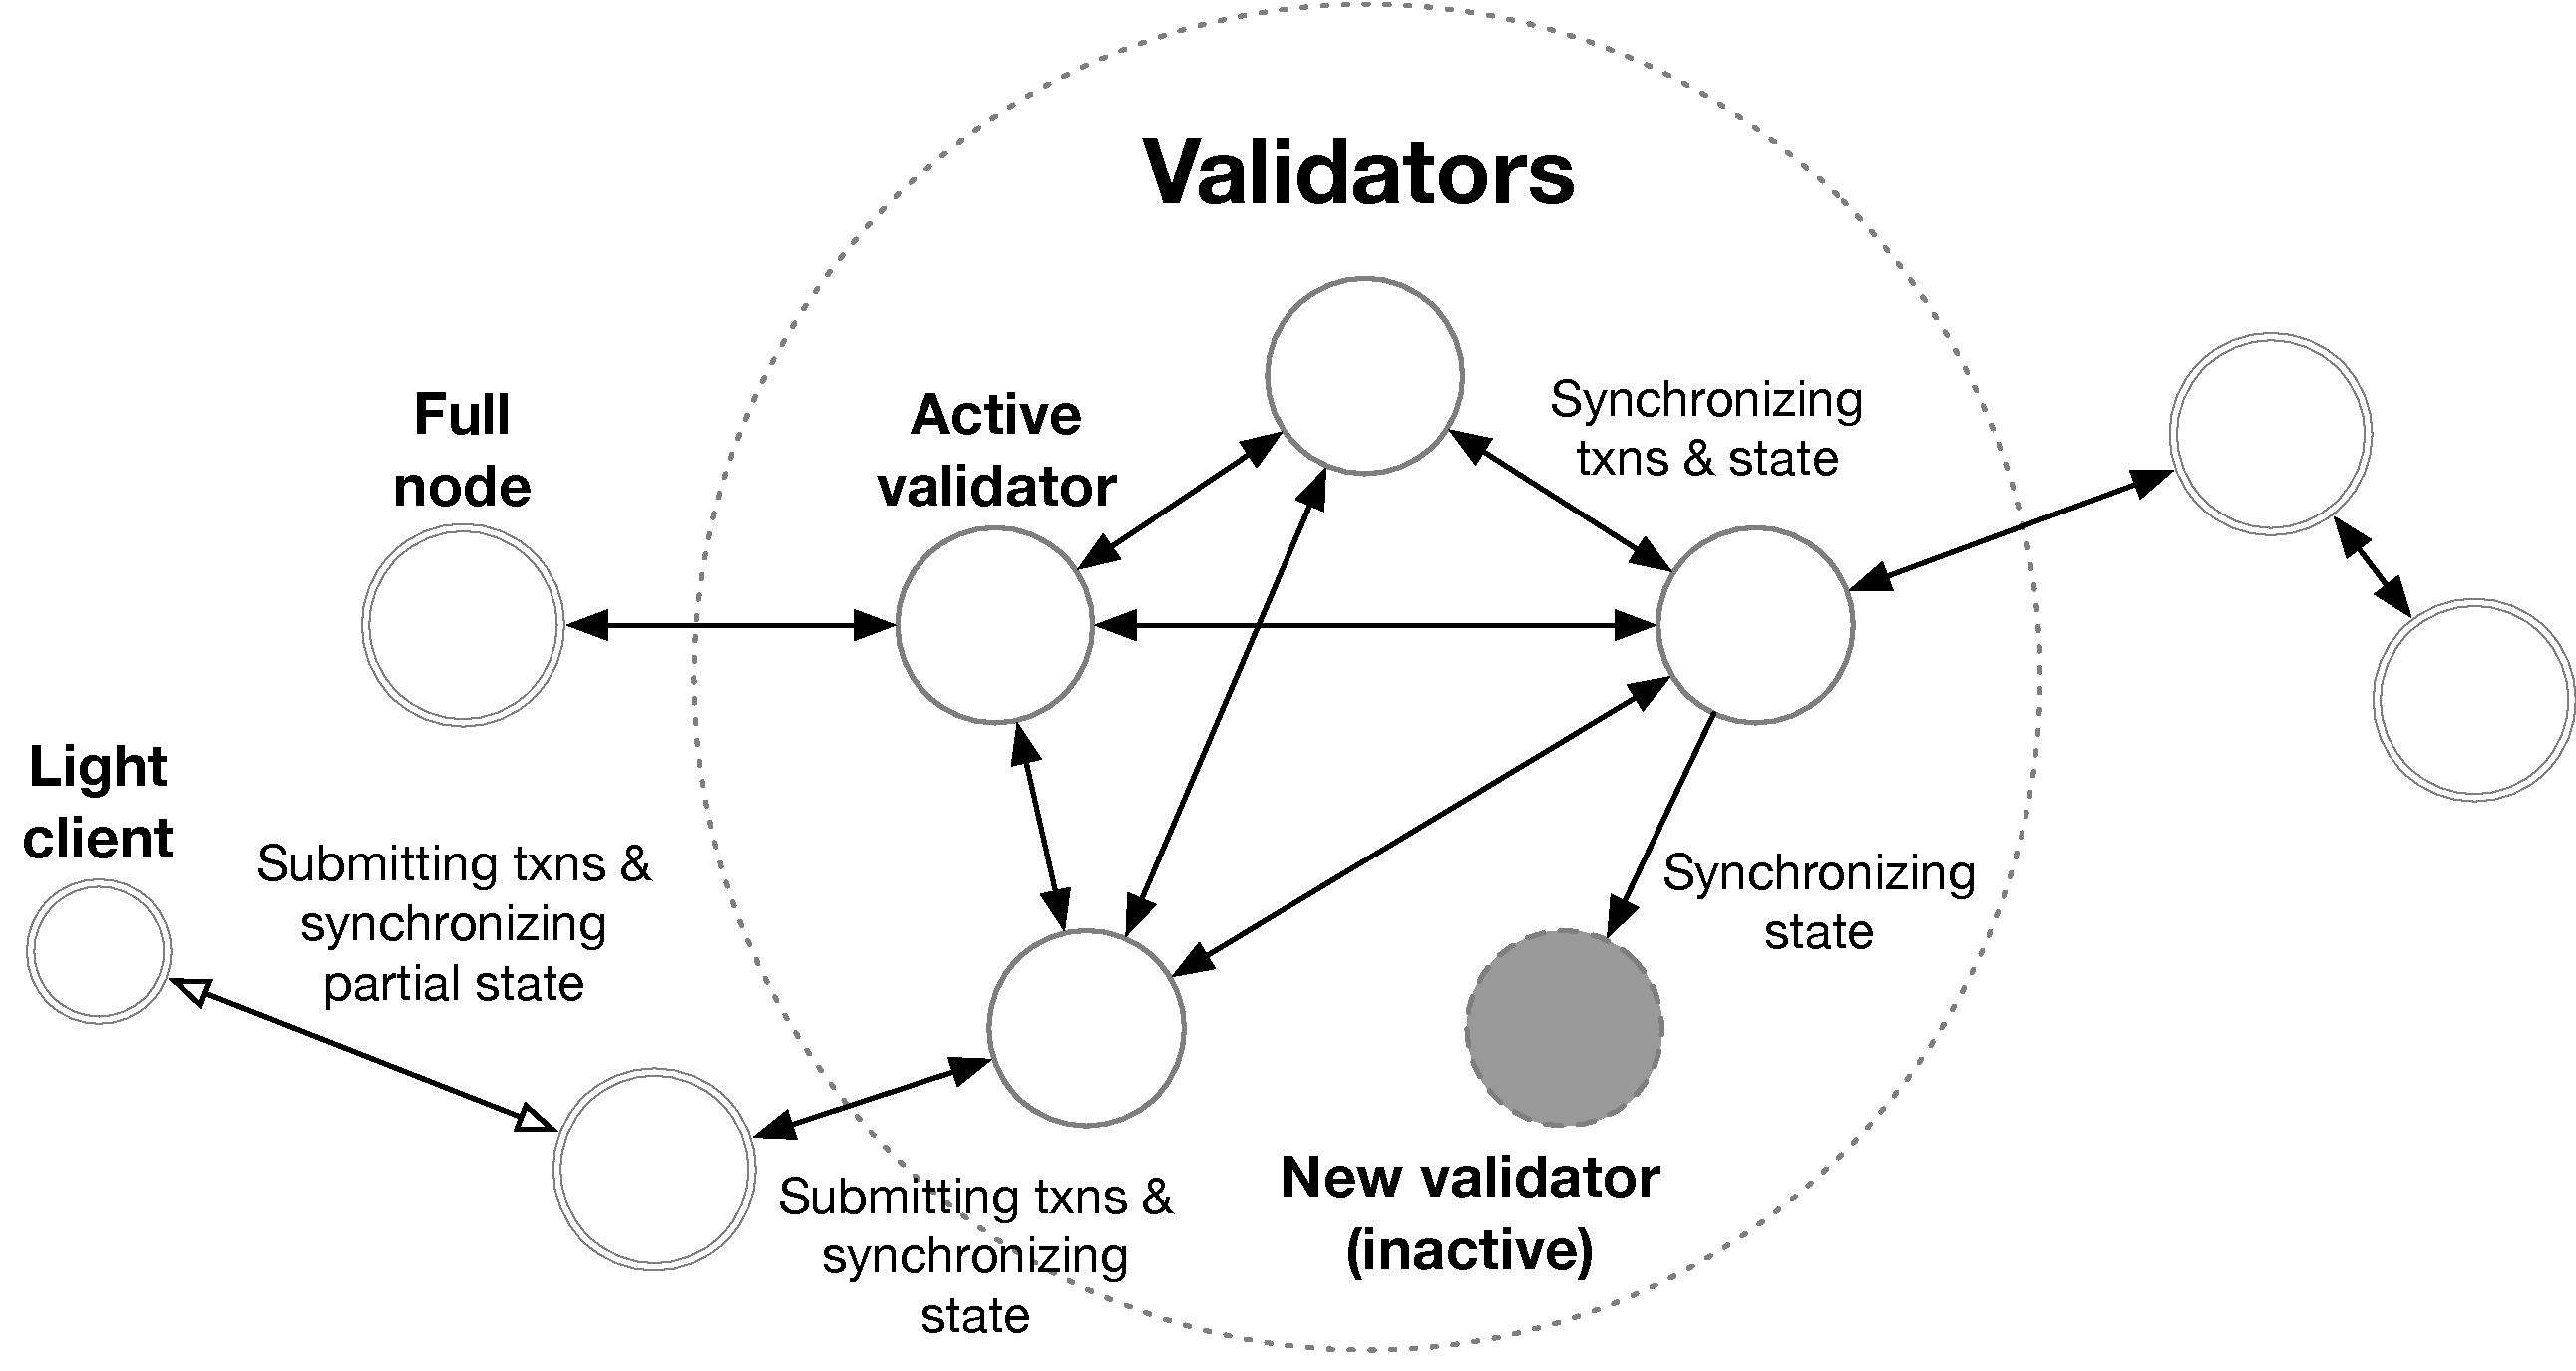
\includegraphics[width=0.9\textwidth]{validators.pdf}
\caption{\label{fig:aptos_ecosystem}Aptos 生态系统的组件}
\end{figure}

\section{概述}
如图 \ref{fig:aptos_ecosystem} 所示,Aptos 区块链由一组验证器( \emph{validators})组成,他们使用拜占庭容错(byzantine fault-tolerant,\emph{BFT}),权益证明(proof-of-stake,POS)的共识机制来接收与处理用户的交易。 代币持有人在他们选定的验证节点(Validator)中锁定或者\emph{质押}他们手上的代币。 每个验证节点的共识投票权重与所质押代币量成正比。 一个验证者可以是\emph{活跃}的状态,并参与到共识决策中。 同样,一个验证节点如果没有足够的质押代币,或被从验证节点集合中轮换出来,亦或在同步区块链状态时离线,再或共识协议因历史表现不佳而拒绝其参与共识,那么该验证节点也可能处于\emph{不活跃}的状态。

\emph{客户端(Clients)}是系统中需要提交交易或查询区块链状态和历史的任何部分。客户端可以选择下载并验证那些被验证节点签署验证过的数据。 

\emph{全节点(Full Node)} 是从验证节点或网络中其他全节点复制交易和区块链状态的客户端。 他们可能会根据需要裁剪掉一些交易历史和区块链状态记录,以重新获得充足的存储空间。 

\emph{轻客户端(Light clients)}只维护当前验证节点的集合,并且可以从全节点中安全地查询部分区块链状态。 钱包是轻客户端的常见例子。
为了满足安全、快速、可靠和可升级的 web3 基础设施的需求,以便被广泛采用,Aptos 区块链基于下列核心设计原则建立:

\begin{itemize}
\item 通过新的智能合约编程语言 Move \cite{move},快速且安全地执行链上逻辑,以及保证简单的可审计性和程序上的可分析性。 Aptos 区块链从 Diem 区块链中继承使用并不断发展 Move。

\item 通过分批、流水线和并行化的交易处理方法实现了极高的吞吐量和低延迟。

\item 与预先识别要读取/写入的数据且破坏交易原子性的现有并行执行引擎不同,Aptos 区块链创新性的使用 Block-STM 技术作为并行执行引擎,有效地支持了任意复杂交易的原子性。

\item 通过快速的、权益质押验证节点的轮换以及对验证节点的信誉跟踪,实现对性能和去中心化治理的优化。

\item 可升级性和可配置性是最重要的设计原则,从而使基础设施可以拥抱新的使用用例和最新的技术。

\item 通过了诸如威胁建模在内的严格的组件级测试和无缝部署的模块化设计,保证了操作的高度安全性和可靠性。


\item 保证去中心化的水平吞吐量可扩展性。源自程序与数据模型的分片(sharding)是水平扩展中的一个重要概念。

\end{itemize}
第 \ref{sec:move} 节解释了开发者如何通过 Move 语言与 Aptos 区块链进行交互。 第 \ref{sec:logical} 节描述了逻辑数据模型。 第 \ref{sec:user} 节详细介绍了 Aptos 区块链如何通过强大的验证方法实现安全的用户体验。 第 \ref{sec:pipelining_batching} 节描述了围绕流水线、批处理和并行化的关键性能创新。 第 \ref{sub:state_sync} 节详细介绍了不同类型的客户端与其他节点同步状态的各种选择。 第 \ref{sec:community_ownership} 章描述了我们对社区所有权和治理的计划。 最后,第 \ref{sec:performance} 节讨论未来在保持去中心化下的性能发展方向。

\section{Move 编程语言}
\label{sec:move}

Move 是一种注重安全和灵活性的新型智能合约编程语言。 Aptos 区块链使用 Move 的对象模型来表示其账本状态(见 \ref{sub:ledger_state} 节),并使用 Move 代码(模块)来编码状态转换的规则。 用户提交的交易中,可以包括发布新模块、升级现有的模块、执行模块内定义的接口功能,以及可以直接与模块的公共接口互动的脚本。

Move 生态系统包含一个编译器、一个虚拟机和许多其他的开发工具。 Move 受到 Rust 编程语言的启发,该语言通过线性类型等概念来明确数据的所有权 Move 强调了资源的稀缺性、保存和访问控制。 Move 模块定义了每个资源的生命周期、存储和访问模式。 这确保了像代币 (\mintinline{rust}{Coin}) 这样的资源不会在没有适当凭证的情况下产生,且不能被重复消费,也不会消失。

即使存在不受信的代码,Move 仍然可以利用字节码验证工具来保证类型和内存安全。 为了帮助编写更可靠的代码,Move 包括了一个类型验证器,Move Prover \cite{move_prover},能够根据给定的规范,验证 Move 程序的功能正确性,该类型验证功能已经集成到了 Move 语言中。

除了用户帐户和相应的帐户内容,分布式账本的状态还包含 Aptos 区块链的链上配置。 这个网络配置包括当前活跃状态的验证节点的集合,质押的属性,以及 Aptos 区块链内各种服务的配置。 Move对模块可升级性和全面可编程性的支持实现了无缝的配置变化,并支持对 Aptos 区块链本身的升级(这两类升级已经在非公开的主网上执行了多次,并且没有宕机记录)。

Aptos 团队已经进一步增加了 Move 的特性,支持更广泛的 web3 用例。 如下文 \ref{sub:ledger_state} 节所述,Aptos 区块链实现了细粒度的资源控制。 这个特性不仅有效支持了并行执行,而且几乎固定了访问与更改数据的成本。 此外,Aptos 区块链提供了建立在细粒度存储之上的表支持,这使得大规模的数据集(例如,大量的 NFT 集合)可以在一个账户中实现。 同时,Aptos 支持完全在链上体现的共享或自动化账户。 这使得复杂的去中心化自治组织(DAO)能够共享账户,以及将这些账户作为异质资源集合的容器。

\section{逻辑数据模型}
\label{sec:logical}

Aptos 区块链的账本状态(\emph{ledger state})代表了链上所有帐户的状态。 账本状态使用一个无符号的 64 位整数进行版本划分,对应与当前系统所执行的交易数量。 任何人都可以向 Aptos 区块链提交交易以修改账本状态。 交易执行后,会生成一个 交易输出 (\emph{transaction output})。 一个交易的输出包含零个或多个操作来操纵账本状态(被称为 \emph{write sets}),一个由此产生的事件集合(见第 \ref{subsub:events} 节),消耗的 gas,以及已执行的交易状态。

\subsection{交易}

一个经过签名的交易包含以下信息:

\begin{itemize}
\item \textbf{交易身份验证器}:发送者使用包括一个或多个数字签名的交易身份验证器来验证交易是否已被验证。
发送方地址
\item \textbf{发送方地址}: 发送方的帐户地址。

\item \textbf{Payload}: Payload 或是指链上现有的接口函数,或是指包含要作为内联字节码执行的函数(称为脚本)。 此外,一组由字节数字编码的参数。 对于点对点交易,输入参数包含接收方的信息和转入金额。

\item \textbf{Gas 价格} (以指定货币/Gas 单位):这是发送方愿意为执行交易而支付的每单位 Gas 的金额。 Gas 费指的是支付计算、联网和存储的费用。 Gas 是一种抽象的计算单位,没有固有的实际价值。

\item \textbf{最大 Gas 单位数(Maximum gas amount)}: 最大 Gas 是在交易中止前允许消耗的最大 Gas 单位数。 帐户内必须至少有 Gas 单价乘以最大 Gas 单位数的余额,否则交易将在验证过程中被终止执行。

\item \textbf{序列号}: 交易的序列号。 交易中的序列号必须与交易执行时发送方帐户中存储的序列号相匹配。 交易成功执行后,将递增账户序列号,以防止重放攻击。

\item \textbf{到期时间}: 一个时间戳,过了这个时间戳,交易将不再有效。

\item \textbf{区块链 ID}: 识别区块链中的交易有效性,为用户提供进一步的保护,防止签署错误。

\end{itemize}
在每个版本 $i$, 状态变化由元组 (tuple) $(T_i, O_i, S_i)$ 表示,分别包含交易、交易输出和交易结束后的账本状态。 给定一个确定性的函数 $\textsf{Apply}$, 执行交易 $T_i$,账本状态 $S_{i-1}$, 产生交易输出 $O_i$ 和新账本状态 $S_i$。 也就是说, $\textsf{Apply}(S_{i-1}, T_i) \rightarrow \langle O_i, S_i\rangle$. 

\subsubsection{事件}
\label{subsub:events}

事件是交易执行过程中发出的。 每个 Move 模块可以定义自己的事件,并选择在执行时何时发出这些事件。 例如,在转账期间,发送方和接收方的账户将分别发出 \emph{SentEvent} 和 \emph{ReceivedEvent}。 数据会存储在账本内,可以通过 Aptos 节点进行查询。 每个注册事件都有一个唯一的索引,该索引可用于查询事件详细信息。

向同一事件索引发出的多个事件会产生事件流(\emph{event streams}),这是一个事件列表,每个条目包含一个从 0 开始依次增加的数字、类型和数据。 每个事件必须以某种类型定义。 会存在多个不同事件由相同或类似的类型定义,特别是在使用泛型的时候。 事件有关联的数据。 对于 Move 模块的开发者来说,通用原则是要包括所有必要的数据,以便理解在交易执行前后引起的底层资源变化,这些变化改变了数据并发送了事件。

交易只能生成事件,不能读取事件。 这种设计使交易的执行只能以当前状态和当前交易的输入作为入参,而不是历史信息(例如,先前生成的事件) 。

\subsection{账户}
\label{sec:accounts}

每个账户都由一个独特的256位数值来识别,称为账户地址。 在账本状态中创建一个新账户 (见 \ref{sub:ledger_state} 节),当现有账户发送交易会调用 \mintinline{rust}{create_account(addr)} Move 函数就可以进行创建。 这通常发生在一个交易试图将 Aptos 代币发送到一个尚未创建的账户地址。 为了方便起见,Aptos 还支持一个 \mintinline{rust}{transfer(from, to, amount)} 函数,如果在转移之前账户不存在,则会隐含地创建一个账户。


要创建一个新帐户,用户首先生成一个签名密钥对:$(vk, sk)$。 接下来,将签名方案标识符 $(ssid)$ 与公钥vk拼接在一起,通过加密哈希 $H$ 得出特定签名方案的新账户地址:即 $addr = H(vk, ssid)$。

在地址 \mintinline{rust}{addr} 处创建新账户后,用户可以签署将从 \mintinline{rust}{addr} 处的账户发送的交易,使用私钥 $sk$ 来签署。 用户还可以轮换 $sk$,可以是主动更改 $sk$ ,也可以是应对可能出现的私钥泄露。 改变私钥的操作不会改变帐户地址,因为帐户地址的创建只来自于公钥

Aptos区块链并不将账户与现实世界的身份联系起来。 一个用户可以通过生成多个密钥对创建多个账户。 由同一用户控制的账户彼此之间没有内在联系。 然而,为了资产管理的简便化,单个用户仍然可以在一个钱包中管理多个账户 这种灵活性为用户提供了匿名性,同时我们在未来的版本中尝试使用更多隐私保护原语(privacy-preserving primitives)。 如 \ref{subsec:parallel_transaction_execution} 节所述,由一个用户或一组用户拥有的多个账户也提供了增加执行并发性的渠道。

\begin{figure}
\centering
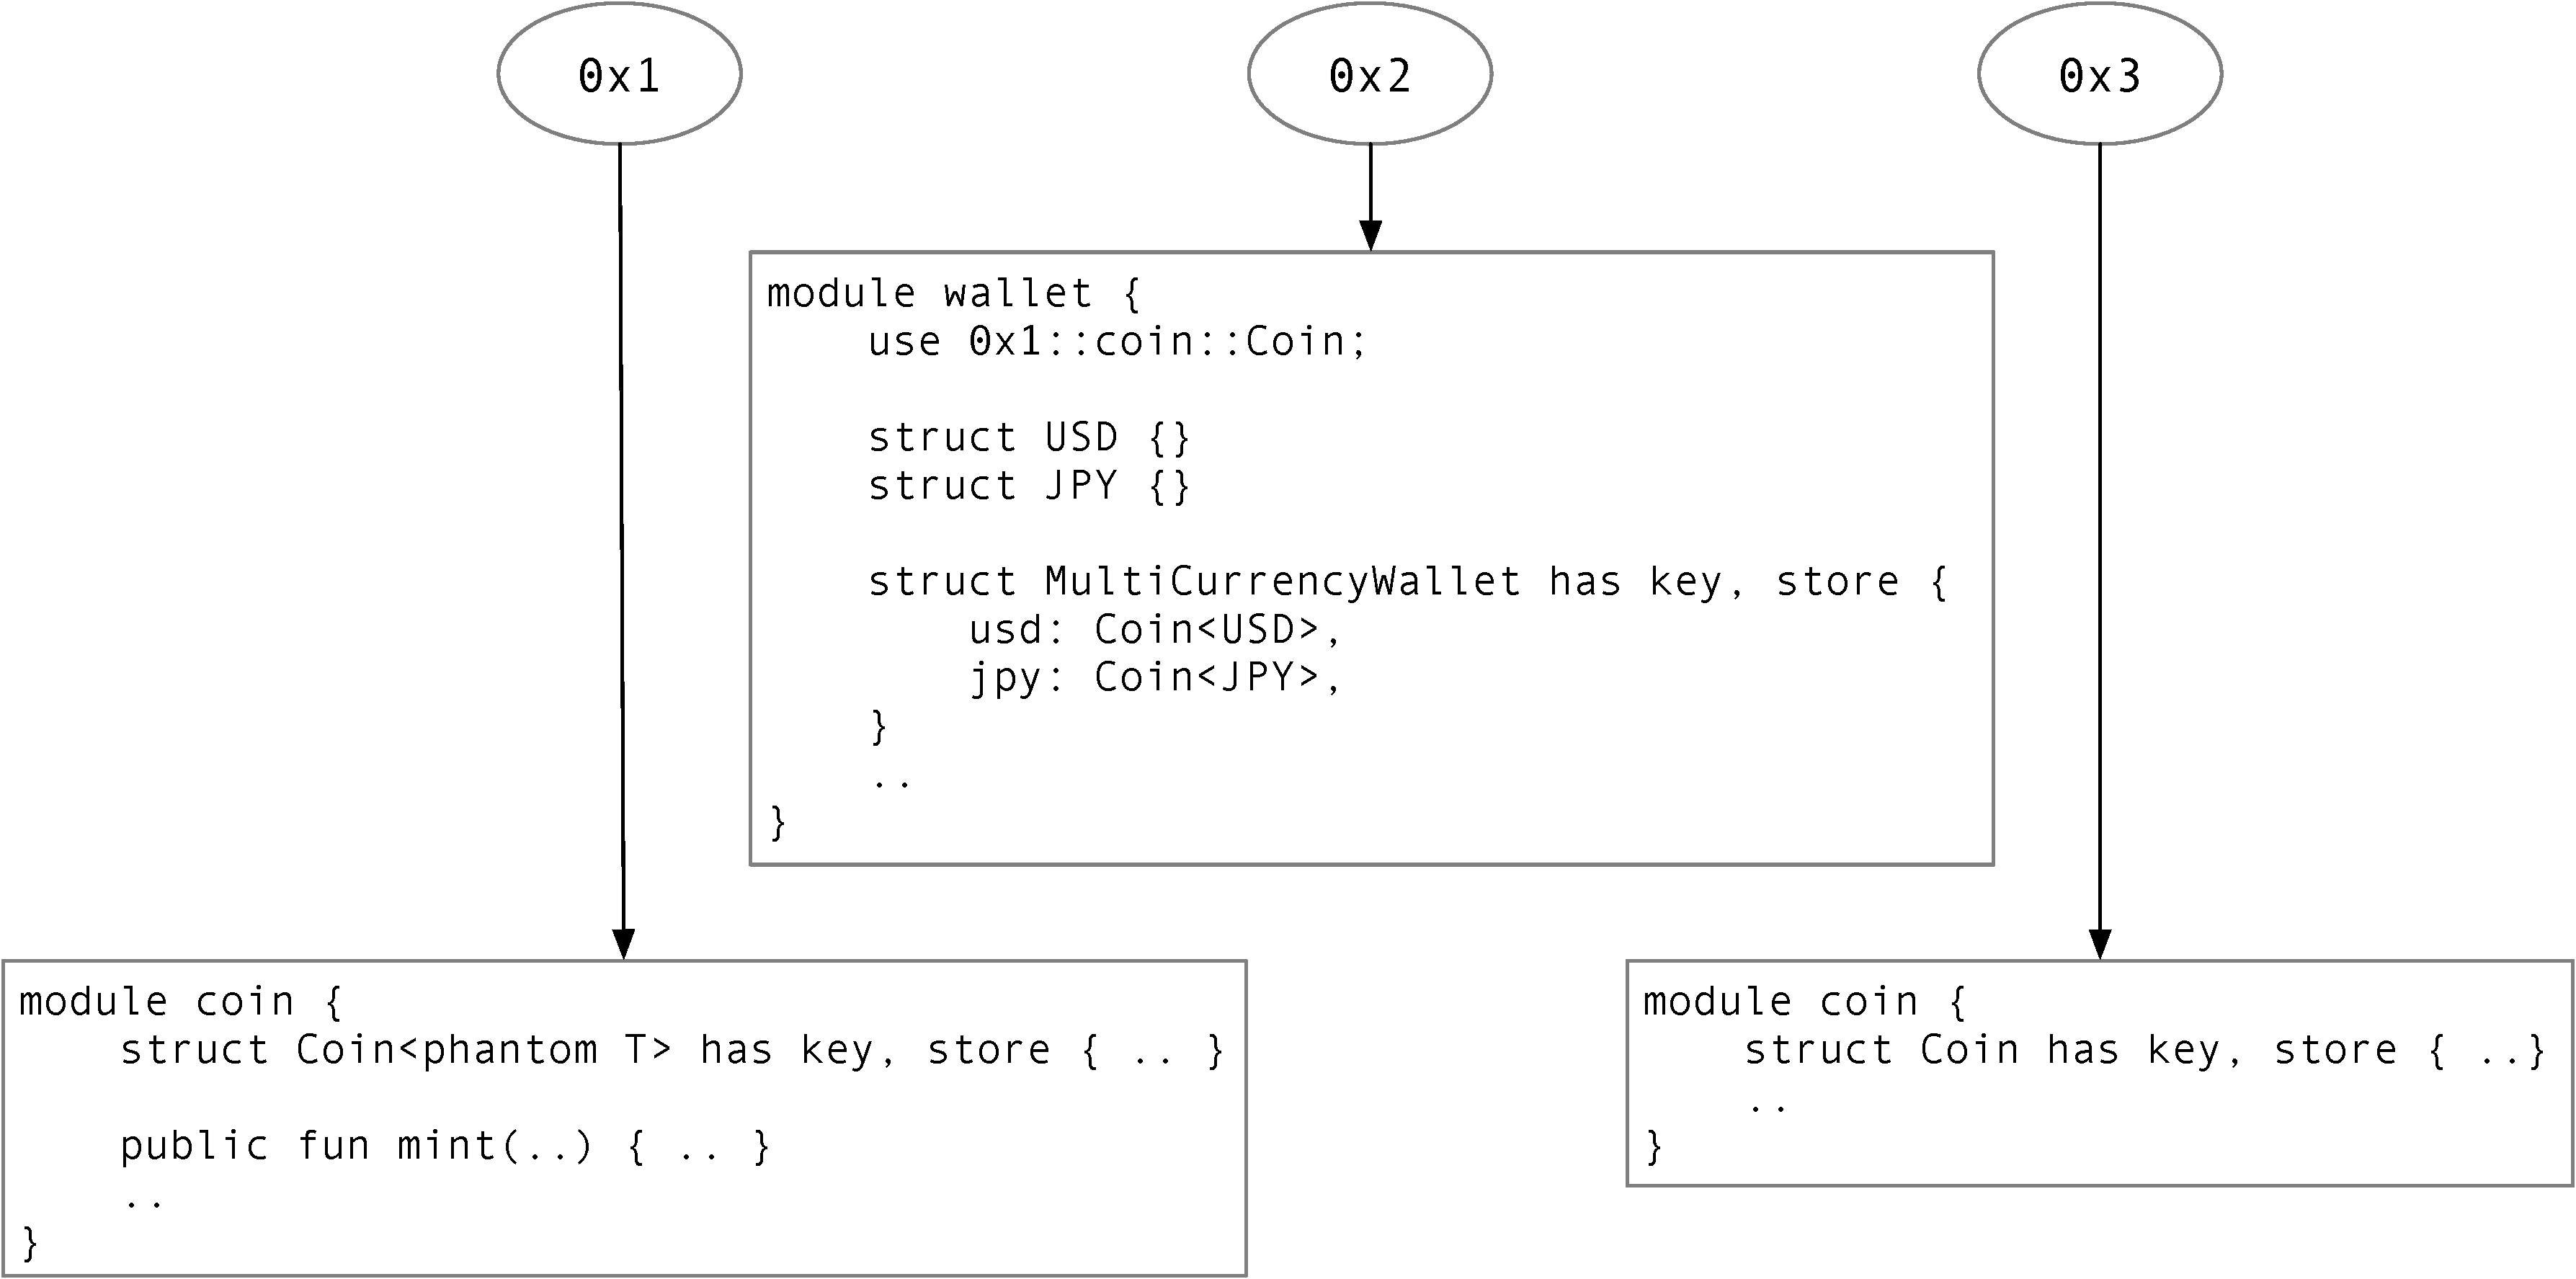
\includegraphics[width=0.85\textwidth]{move_1.pdf}
\caption{\label{fig:move_modules}链上 Move 模块示例}
\end{figure}

\subsection{Move 模块}

一个 Move 模块包含声明数据类型 (structs) 和程序的 Move 字节码。 它是由声明模块的账户地址和模块名称一起标识的。 例如,图 \ref{fig:move_modules} 中第一个货币模块的标识符是 \mintinline{rust}{0x1::coin}。 一个模块可以依赖于其它链上模块,如图 \ref{fig:move_modules} 中的钱包模块所显示,可以复用其他模块的代码。

一个模块在一个账户内必须是唯一的,也就是说,每个帐户下模块名称必须保持唯一性。 例如,图 \ref{fig:move_modules} 中地址为 \mintinline{rust}{0x1} 的账户无法声明另一个名为 \mintinline{rust}{coin} 的模块。 另一方面, 地址为 \mintinline{rust}{0x3} 的帐户可以声明一个名为 \mintinline{rust}{coin} 的模块,这个模块的标识符将是 \mintinline{rust}{0x3::coin}。 注意, \mintinline{rust}{0x1::coin::Coin} 和 \mintinline{rust}{0x3::coin::Coin} 是不同的类型,不能互换使用,也不共享公共模块代码。 相反,\mintinline{rust}{0x1::coin::Coin<0x2::wallet::USD>} 和 \mintinline{rust}{0x1::coin::Coin<0x2::wallet::JPY>} 是同一通用类型的不同实例,不能互换使用,但可以共享公共模块代码。

相同地址下的模块将会被归并到同一个软件包(\emph{packages})中 此地址的所有者将软件包作为一个整体进行链上发布,包括字节码和软件包元数据。 软件包的元数据决定一个软件包是可以升级的还是不可改变的。 对于可升级的软件包,在允许升级之前会进行兼容性检查:不能改变现有的接口函数,也不能在内存中储存任何资源。 但是,升级可以添加新的函数和资源。

Aptos框架由Aptos区块链的核心库和配置组成,被定义为一个可定期升级的模块包 (见 \ref{subsec:network_governance} 节) 。

\subsection{资源}
\label{subsec:resources}

与模块类似,账户地址也可以有与之相关的数据。 在每个账户地址中,数据值是由其类型决定的,每个账户下,每种类型的数据值都应保持唯一。 以图 \ref{fig:move_data} 为例, 地址 0x50 持有一个单一值,其中 \mintinline{rust}{0x3::coin::Coin} 是完全限定的类型。 \mintinline{rust}{0x3} 是存储 coin 模块的地址, \mintinline{rust}{coin} 是模块的名称, \mintinline{rust}{Coin} 是数据类型的名称。 也可以使用泛型数据值,不同的泛型实例被视为不同的类型。 这对可扩展性至关重要,允许不同的实例共享相同的功能代码。

变更、删除和发布一个数据的规则被编码在定义数据类型的模块中。 Move 的安全和验证规则防止其他代码或实体直接创建、修改或删除其他模块中定义的数据类型的实例。

一个地址下的每种类型最多只有一个顶层值,这听起来似乎很有局限性。 然而,这在实践中并不是一个问题,因为开发者可以通过定义不同的封装类型,将相同类型数据作为成员变量,从而避免了任何限制。 \mintinline{rust}{Wallet} 结构 (位于图 \ref{fig:move_data} 中) 就是一个如何使用包装器类型的例子。

还应该注意的是,并非所有数据类型都能在链上储存。 为了使数据实例有资格成为顶层值,数据类型必须具有 \mintinline{rust}{key} ability。 同样,对于嵌套的值来说,\mintinline{rust}{store} 能力是必需的。 具有两种能力的数据类型也被称为资源 (\emph{resources})。


\begin{figure}
\centering
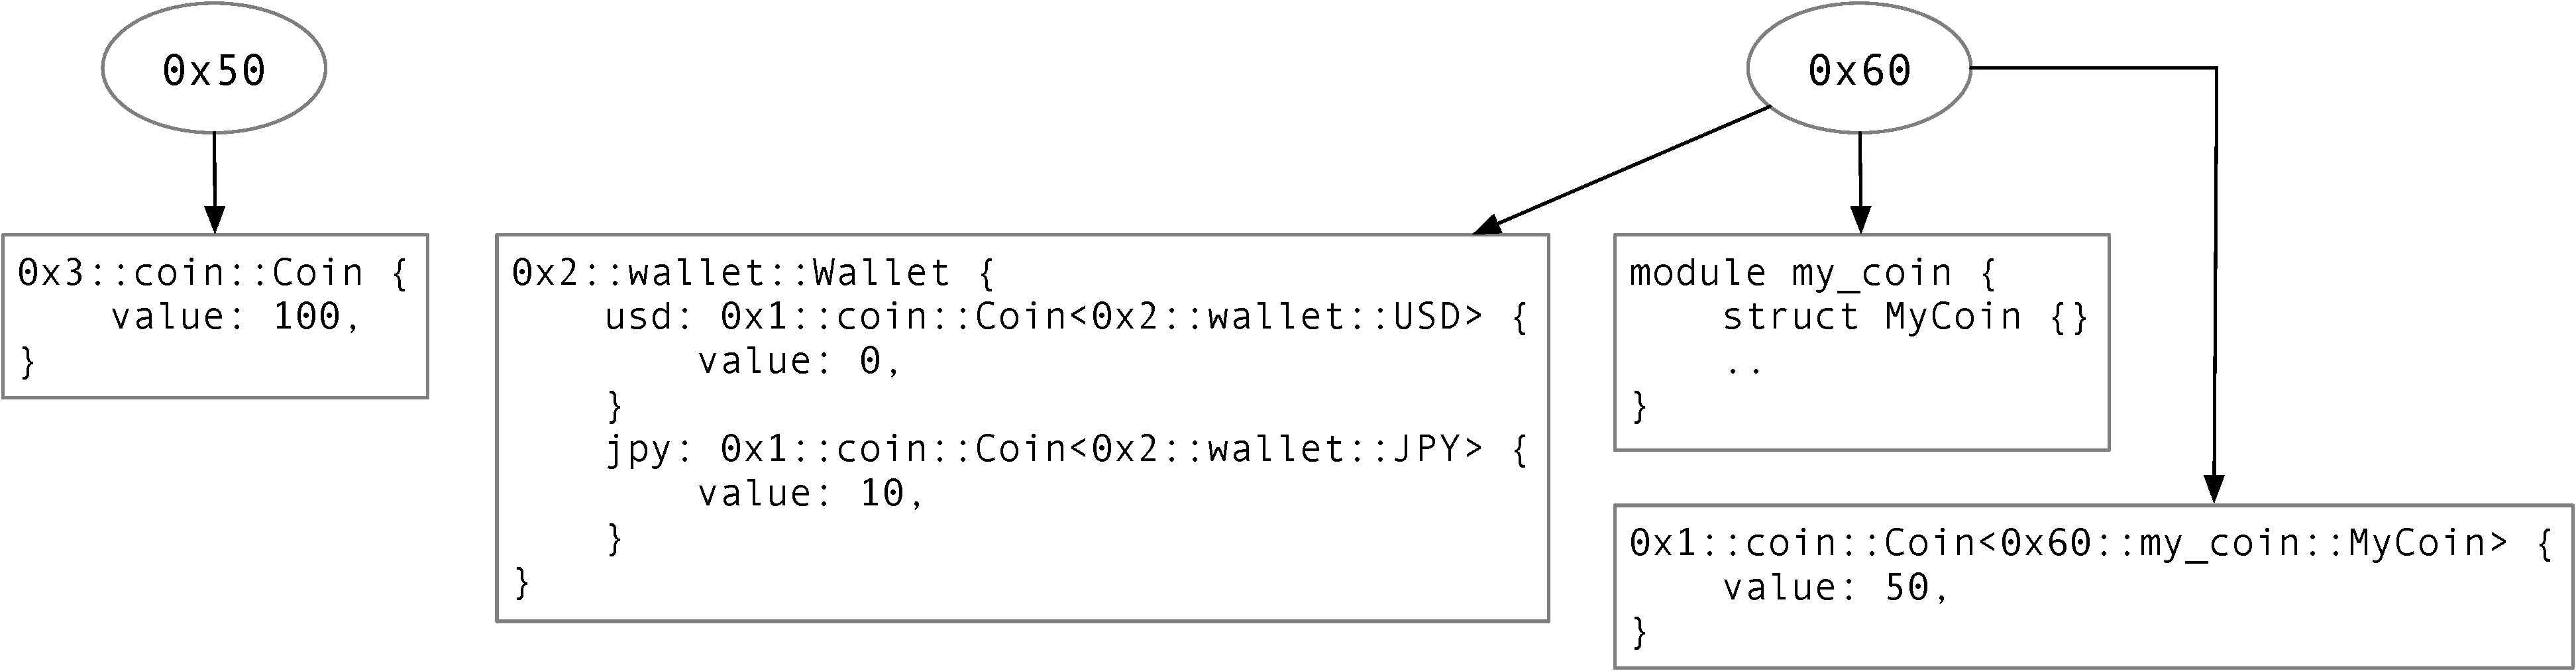
\includegraphics[width=1.0\textwidth]{move_2.pdf}
\caption{\label{fig:move_data}链上数据示例}
\end{figure}


\subsection{账本状态}
\label{sub:ledger_state}

从 Move 虚拟机 (Move VM) 的角度来看,每个账户都由一组值和 key-value 数据结构组成。 这些数据结构被称为表项 (\emph{table entries}),并以二进制规范化序列化格式 (BCS) 存储。 这种数据结构设计可以使开发者编写在少量数据复制到大量账户的场景下,可以高效执行的智能合约;也可以编写大量数据集中在少量账户上场景下,可以高效执行的智能合约。 Move 模块的存储方式与账户数据类似,但在一个独立的命名空间下。 创世账本状态定义了区块链初始化时的初始账户集及其相关状态。

在启动时,Aptos 区块链将由一个单一的账本状态表示。 然而,随着使用的普及和技术的发展,Aptos 将扩大分片的数量,以提高吞吐量 (即启用多个账本状态) ,并支持跨分片移动或访问资产的交易。 每个账本状态将维护特定分片的所有链上资产,并提供相同的账户模型,以及细粒度的 key-value 数据存储,为存储访问提供近乎固定的成本。

\section{安全的用户体验}
\label{sec:user}

为了覆盖数十亿互联网用户,web3 的用户体验必须是安全便捷的。 在本章节中,我们将描述 Aptos 区块链为实现这一目标的几项创新。


\subsection{交易可行性保护}
\label{subsec:transaction_replay_protection}

签署交易意味着签名者授权区块链提交和执行该交易。 有时候,用户会在不小心或者没有意识到交易会被操控的情况下签署交易。 为了减少这种风险,Aptos 区块链对每笔交易的可行性进行限制,并保护签名者避免陷入无限确认的操作中。 目前 Aptos 提供了三种不同的保护措施:发送者的序列号、 交易过期时间和指定的链标识符。

\begin{itemize}
\item 交易的序列号对于每个发送者的帐户只能提交一次。 因此,如果发送者发现当前账户序列号 $\geq$  交易 $t$ 的序列号,那么 $t$ 已经被提交,或 $t$ 永远不会被提交(因为 $t$ 使用的序列号已经被另一个交易占用)。

\item T区块链时间以高精度和高频率 (通常为亚秒) 推进,详情见 \ref{subsubsec:blockchain_time}。 如果区块链的时间超过交易 $t$ 的到期时间,那么同样的,要么 $t$ 已经被提交,要么 $t$ 永远不会被提交。

\item 每笔交易都有一个指定的链 Id,以防止恶意实体在不同区块链环境之间进行重放攻击 (例如,跨测试网和主网)。

\end{itemize}

\subsection{基于 Move 的密钥管理}

正如 \ref{sec:accounts} 节所述,Aptos 帐户支持密钥轮换(key rotation),这是一个重要的特性,可以降低私钥泄漏,远程攻击以及现有密码算法未来被破解的风险。 此外 Aptos 的账户也足够灵活,可以支持新的混合托管模型, 用户可以将轮换帐户私钥的能力委托给一个或多个托管方以及其他可信实体。 然后通过 Move 模块定义一个策略,使这些受信实体能够在特定情况下轮换密钥。 例如, 实体可能是由许多受信任方持有的 $k$-out-of-$n$ 多签密钥,从而可提供密钥恢复服务以防止用户密钥丢失(例如,20\% 的比特币目前被锁定密钥丢失的帐户中 \cite{lost_passwords} )。

此外,虽然许多钱包提供诸如云端备份私钥,多方计算和社会恢复等多种密钥恢复方案,但这些方案并非基于区块链实现(即链下的)。 因此,每个钱包都要实现自己的密钥管理方案,对用户而言,密钥的管理变成了黑盒。 相反, Aptos 中的密钥管理功能提供了完整透明的密钥管理操作,同时极大地降低了了实现钱包密钥管理方案的难度。

\subsection{预签名交易透明度}

如今,钱包对其所签署的交易几乎是不透明的。 因此,经常有户被恶意交易欺骗,导致资金损失以及一系列严重的后果。 即使是可以查询到每笔链上交易数据的区块链也无法避免这种损失。 目前几乎没有用户保障措施,使得用户暴露于各种各样的攻击之下。

为了解决这个问题, Aptos 生态系统提供了交易预执行服务 (\emph{transaction pre-execution}):可在用户签名之前 向他们提供交易结果(以人类可读的形式)。 Aptos 将交易预执行服务与以往已知的攻击和恶意智能合约相结合,将有助于减少欺诈。 此外,Aptos 还允许钱包在执行过程中规定对交易的限制。 违反这些限制将导致交易被中止,以进一步保护用户免遭恶意应用程序或社会工程攻击。

\subsection{实用的轻客户端协议}

仅仅依靠 API 提供商的 TLS/SSL 证书在区块链客户端和服务器之间建立的信任并不能充分保护客户端。 即使存在有效证书,钱包和客户端也无法保证所提供数据的真实性和完整性给他们。 因此,API 提供商可能会返回错误或恶意区块链数据,欺骗第三方并进行双花攻击。

为了防止这种情况发生,Aptos 提供状态证明和轻客户端验证协议,钱包和客户端可以使用这些协议来验证由不可信的第三方服务器提供的数据的有效性。 此外,如 \ref{subsubsec:period_state_certification} 所述,使用基于时间戳的状态证明,轻客户端可以通过跟踪网络配置中的变化(\emph{epoch 变更}) 或从当前受信任的节点(锚点 \emph{waypoints})同步最新状态 \cite{waypoints},来保证账户状态的实时性(例如,在几秒钟内)。 通过高频时间戳和低成本状态证明的结合,Aptos 为客户提供了安全的服务。

此外,Aptos 节点还提供了丰富的高性能存储接口,未来进一步微调这些接口后,支持订阅链上特定数据和帐户的证明。 这可以让轻客户端日后仅保留最小的可验证数据,而无需运行一个完节点或处理大量的交易。


\section{流水化、批量、并行的交易处理}
\label{sec:pipelining_batching}

为了最大限度提高吞吐量,增加并发性,并且降低工程复杂性,Aptos 区块链的交易处理过程被划分为不同的阶段。 每个阶段都是完全独立的并且可以各自并行,类似于现代的超标量处理器架构。 这不仅提供了显著的性能优势,而且让 Aptos 区块链能够提供新的验证者-客户端交互模式。 例如:

\begin{itemize}
\item 当指定交易被包含在一批留存交易中,客户端会被通知。 已留存且有效的交易一般会被立即提交。 

\item 当一批已留存交易被排序时,客户端会被通知。 因此,为了减少确定要执行的交易结果的延迟,客户端可以在本地执行交易,而不是等待远程验证节点的完成执行。

\item 客户端可以选择等待验证者执行已认证的交易,然后同步已执行完成的交易状态 (见第 \ref{sub:state_sync} 节) 。

\end{itemize}

Aptos 模块设计有助于提高开发速度以及更短的发布周期,开发者可以对单个模块而不是整个系统进行优化。 类似地,模块设计提供了一条扩展验证器的结构化路径,可以让验证器利用多台机器的计算、网络和存储资源。 图 \ref{fig:pipeline} 交易处理生命周期。


\begin{figure}
\centering
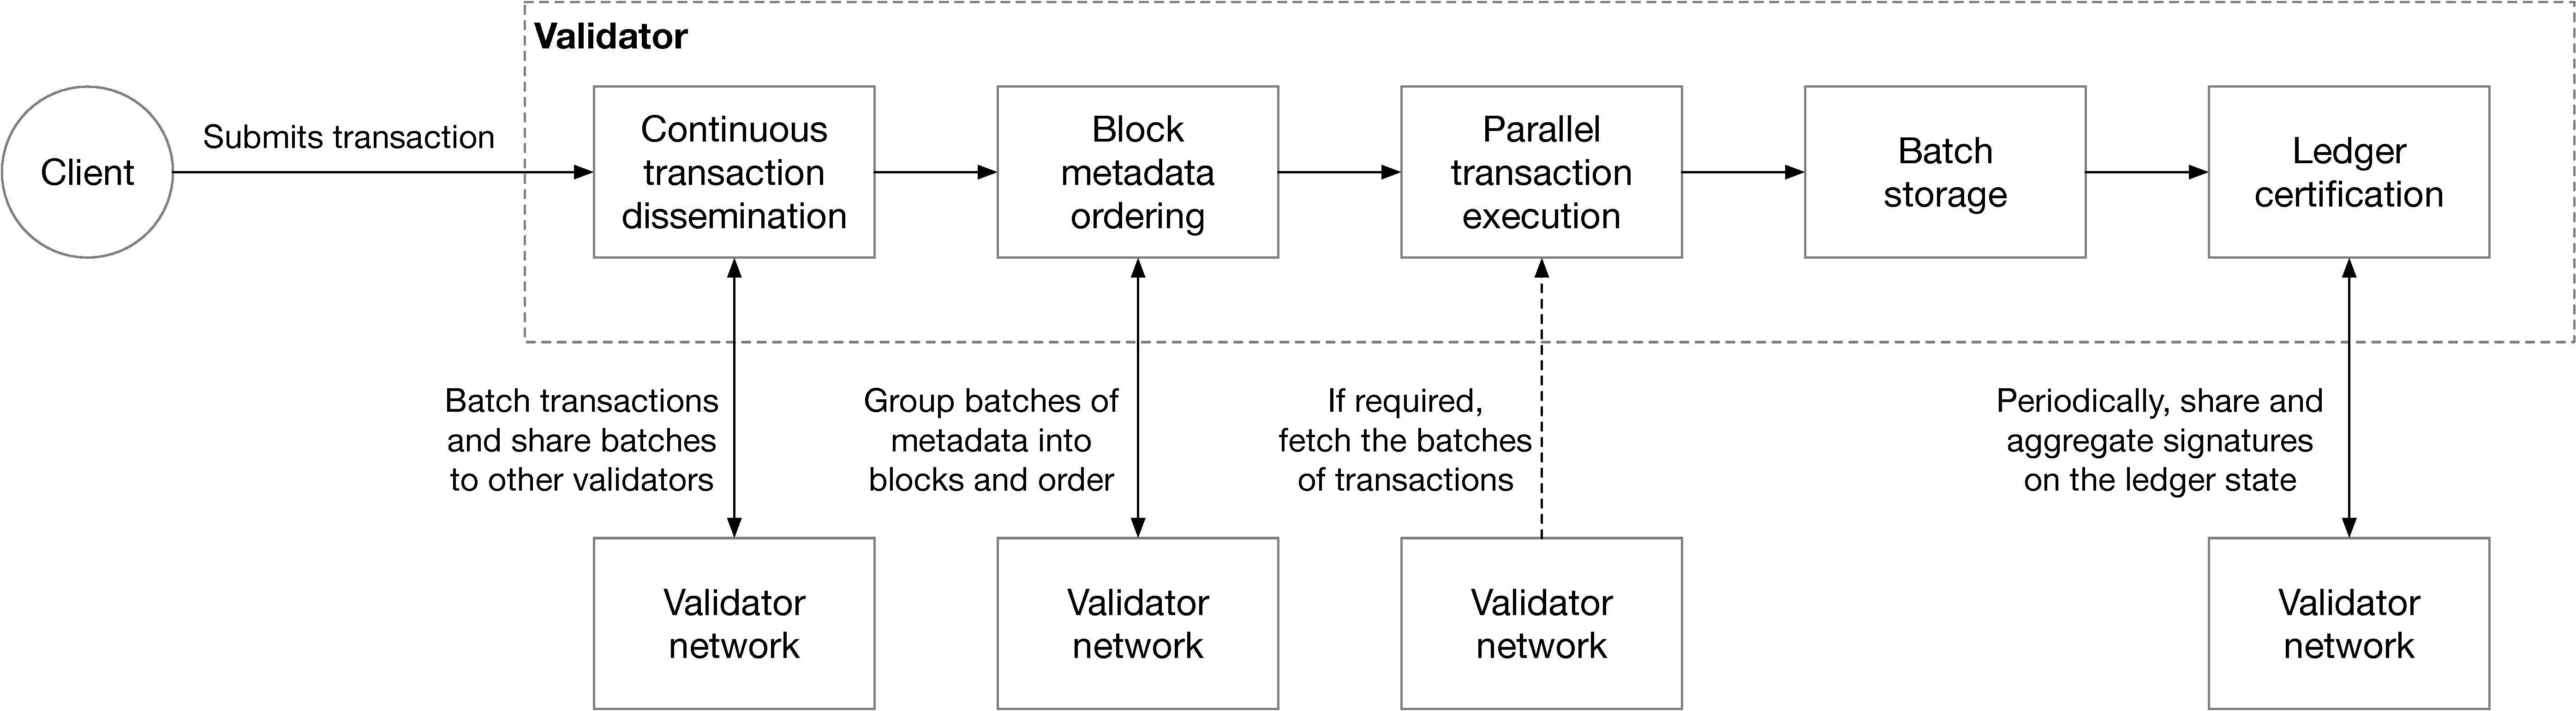
\includegraphics[width=1.0\textwidth]{pipeline.pdf}
\caption{\label{fig:pipeline}交易处理生命周期, 所有阶段都是完全独立的,并且可以各自并行}
\end{figure}

\subsection{批量处理}

批量处理是一个对 Aptos 每个处理阶段都很重要的效率优化。 在广播交易时,验证节点将交易分组为批;在共识阶段将批合并成区块。 执行、存储和账本认证阶段同样批量操作,能为重排序、减少操作( 例如:重复计算或签字验证) 和并行执行提供机会。

将交易打包成批可能会产生少量延迟,例如在传播交易前需等待 200ms 来凑满一批交易。 然而,成批的最长等待时间与最大成批数量是可配置的,使去中心化网络可以自动优化延迟和效率。 批量处理支持高效的费用市场对交易优先级排序,同时避免了恶意客户端造成拒绝服务 (DoS) 攻击。

\subsection{持续的交易广播}
\label{continuous_txn_dissemination}

根据 Narwhal \& Tusk \cite{narwhal_tusk} 的主要观点,Aptos 中交易传播与共识解耦。 验证者不断地相互传输批量交易,同时利用所有可用的网络资源。 验证者 $v$ 分发的每个批次都被持久化,并且将批次摘要的签名发送回 $v$。 根据第 \ref{subsec:block_metadata_ordering} 节中定义的共识要求,任何在批次摘要上的 $2f+1$  个权益加权签名形成可用性证明 (PoAv) 。 这样的证明(PoAv)保证至少有 $f+1$  个加权的诚实验证者已经存储了该批次,因此所有诚实验证者都能够在执行之前检索到它。

无限的待留存交易可能会造成 DoS 攻击,导致验证者节点耗尽存储并崩溃。 为防止这种情况,每批交易都有一个相关的时间戳。 批次上的时间戳可以让验证节点进行高效的垃圾回收。 此外,还设计了一个针对单验证节点的配额机制,确保即使在最极端的情况下 (例如潜在的拜占庭攻击) , 也不会耗尽空间。 同时,批次有数据量限制,Aptos 会在持久化存储校验数据大小。 最后,通过一些对交易缓存和冗余交易数据清理的优化,不仅降低了存储成本,也保证了并行执行引擎的高性能集成。


\begin{figure}
\centering
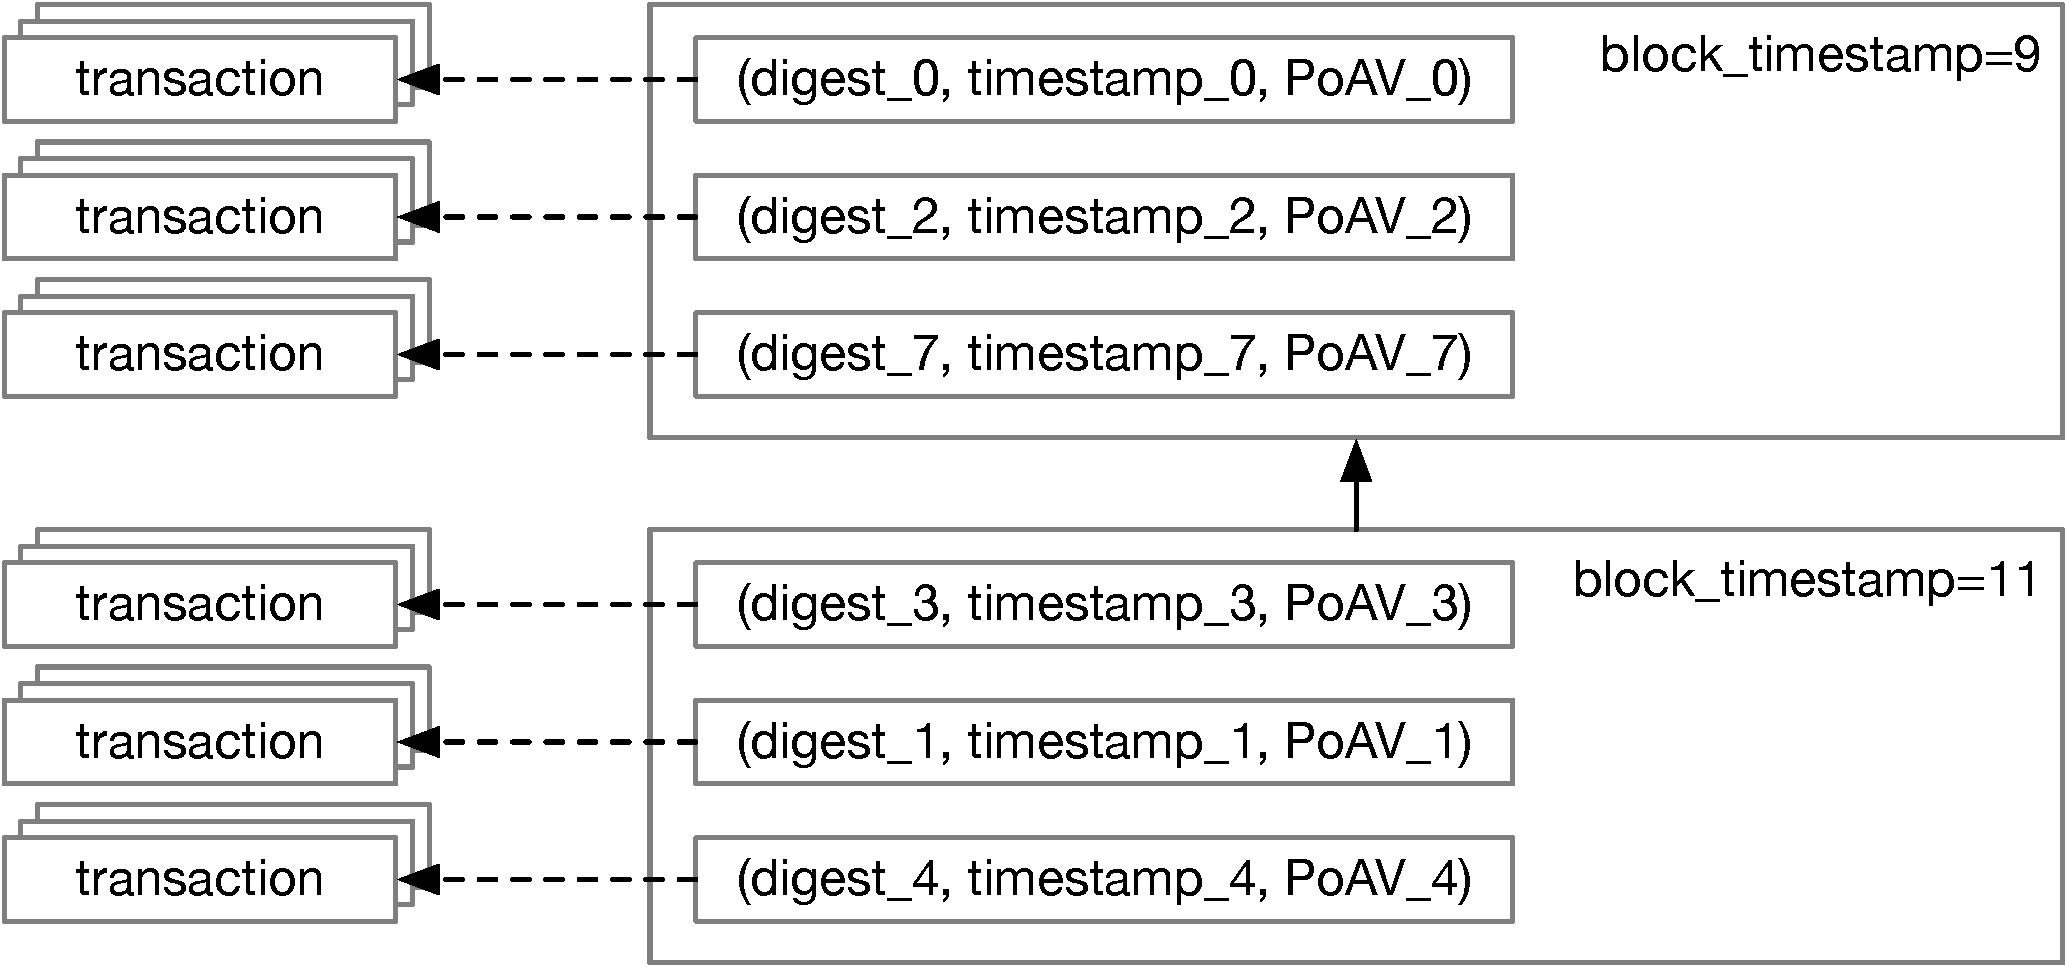
\includegraphics[width=0.8\textwidth]{ordering.pdf}
\caption{\label{fig:block}区块元数据排序独立于广播交易}
\end{figure}

\subsection{区块元数据排序}
\label{subsec:block_metadata_ordering}

存在一种常见的误解:缓慢的共识速度是区块链高吞吐量和低延迟的主要瓶颈。 Aptos 区块链的关键创新之一是将非协议相关的任务从共识阶段解耦出来,例如交易传播、交易执行/存储和账本认证。 通过将交易传播与共识阶段解耦,可以在极低的带宽下进行排序 (仅限区块元数据和证明) ,从而实现交易高吞吐量和最小化延迟。

如今,Aptos 区块链采用 DiemBFTv4 \cite{diembft_v4} 的最新版本,这是一种乐观响应性 BFT 共识协议。 通常,共识只需要两次网络往返 (全网往返时间通常小于 300 毫秒) ,并通过领导者信誉机制动态调整异常验证者 \cite{be_aware}。 链上领导者信誉机制将提升在“窗口期”中成功提交区块的验证器信誉,并对未参与的验证器降级。 这种新颖的机制显著提高了去中心化系统的性能,为节点提供了适当的激励,并将不活跃的验证者对吞吐量和延迟的影响降至最低。

DiemBFTv4 保证部分同步下的活跃性,并确保异步下的安全性,在总验证者权益大于等于 $\geq 3f+1$ 时, 最多可以存在 $f$ 个权益加权错误验证者。 自 2019 年以来,DiemBFTv4 已经在多次迭代中经历数十个节点运营商和多钱包生态系统的广泛测试。 我们还在试验我们最近的研究 (例如 Bullshark \cite{bullshark}) 和其他依赖区块历史和相关通信,以确定区块元数据排序和最终性的协议。

共识区块和提案时间戳由领导者提出并由其他验证者同意,如图 \ref{fig:block} 所示。 需要注意的是,每个共识区块仅包含批处理的元数据和证明。 共识区块中不需要实际交易,因为 PoAV 确保交易批次在区块元数据排序后的执行阶段可用 (参见第 \ref{continuous_txn_dissemination} 节)。 在证明被验证并且满足区块元数据标准 (例如,提议时间戳 $\le$ 区块到期时间) 后,验证者可以对领导者的提议进行投票。

\subsubsection{区块链时间}
\label{subsubsec:blockchain_time}

Aptos 区块链为每个提案的区块以及该区块内相应的所有交易赋予一个近似的,约定的物理时间戳。 此时间戳支持大量重要的使用案例。 例如:

\begin{itemize}
\item 智能合约中与时间相关的逻辑。 例如,开发人员希望编码必须在周四中午12点之前收到一场拍卖的所有出价。
\item 随着预言机发布链上数据,需要准确且可信的链上时间戳来关联事件,并处理来自现实世界数据的延迟。

\item 客户端可以辨别他们在区块链方面的最新情况。 出于安全原因,为避免过时数据和远程攻击,客户端应该能够访问帐户状态更新时间的高精度时间戳。

\item 使用可信时间戳审计区块链可以提供与链下事件的强相关性,例如确保合法强制执行的支出是符合预期要求的。
\item 交易到期是基于最近提交的时间戳。 作为对客户端交易的额外保护,客户端可以选择交易的到期时间,如第 \ref{subsec:transaction_replay_protection} 节所述。

\end{itemize}

Aptos 区块链为区块内所有交易的时间戳提供以下保证:

\begin{itemize}
\item 
在区块链中是时间戳单调递增的。 假设区块 $B1 < $  区块 $B2$,则 $B1$ 上的时间戳 $< B2$ 上的时间戳。

\item 如果一个交易区块的时间戳 $T$ 被认定,那么至少有 $f+1$ 个诚实的验证者认为该时间点 $T$ 已经过去了。 诚实的验证者只会在自己时钟 $\ge$ 区块时间戳 $T$ 时,才能对区块进行投票。 参见第 \ref{continuous_txn_dissemination} 节。
\item 如果一个交易区块一定数量对时间戳 $T$ 的共识签名,那么诚实的验证者直到自己时钟 $\ge$ 时间戳 $T$ 时,才会将此类区块提供给其他验证者。

\end{itemize}

最近的时间戳在每个提交的区块上更新并用作该区块中所有交易的时间戳。 当网络同步时,每次网络往返都会提交一个交易区块,并提供快速更新和高度可靠的时间。 如果需要,可以确定交易区块内更细粒度的排序。


\subsection{并行交易执行}
\label{subsec:parallel_transaction_execution}
一旦对共识区块元数据进行排序,任何验证者节点、完整节点或客户端都可以执行交易。 至少有 $2f+1$  个加权验证者对提案的批次进行了可核查的持续交易。 由于交易传播是连续的,其它的诚实验证者将随着时间的推移接收交易批次。 如果诚实的验证者节点在到达执行阶段时,还没有收到排序批次的交易,那么它可以从 2f+1 个权益加权验证者处下载它们,已知至少有 $f+1$ 个权益加权验证者 ( $\ge$ 一半的权益加权 PoAV 签名者) 是诚实的。

区块链的一个重要目标是实现尽可能多的并行处理。 Aptos 区块链从数据模型和执行引擎两方面着手。

\subsubsection{并行数据模型}

Move 语言数据模型本身支持数据和模块的全局寻址。 数据和账户不重叠冲突的交易可以并行执行。 鉴于 Aptos 中使用了流水线设计,交易的重排序可以减少冲突,从而提高并发性。

即使交易修改了同一组链上值,大部分的交易仍可并行执行。 Aptos 区块链引入了一个新概念,\emph{delta writes},它描述了对账户状态的修改,而不是修改后的账户状态(例如,增加一个整数而不是简单地确定最终值) 。 所有交易处理都可以并行完成,然后以正确的顺序对冲突值进行 delta writes 操作,以确保确定性结果。

随着时间的推移,Aptos 区块链将继续通过提高并发性(例如,利用读/写提示)以及改善开发体验的方式来增强数据模型,让开发人员更自然地创建、修改和组合链上值。 Move为语言级别和平台特定功能上的改进提供了灵活性。

\begin{figure}
\centering
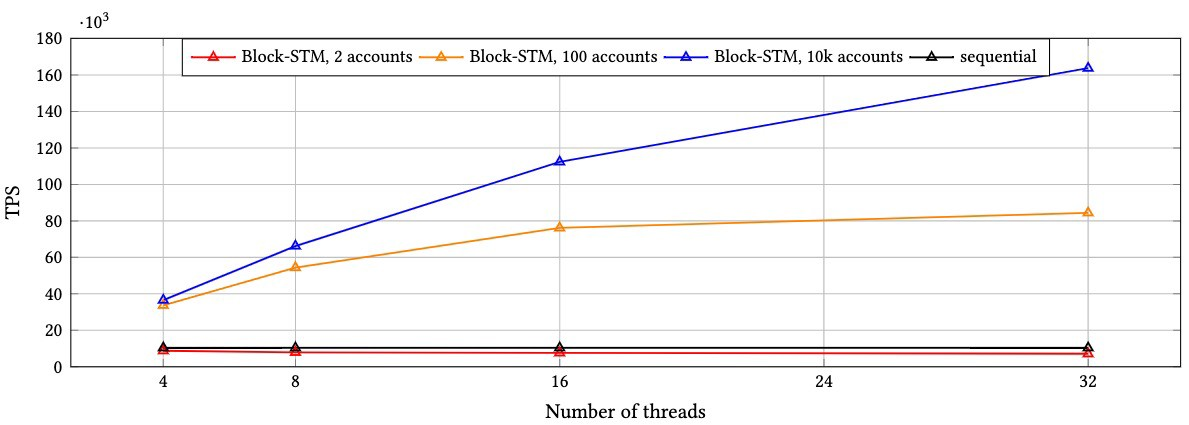
\includegraphics[width=0.95\textwidth]{perf.jpg}
\caption{\label{fig:perf}Block-STM (仅该组件) 不同竞争程度与不同CPU核数下的基准测试}
\end{figure}

\subsubsection{并行执行引擎}

Block-STM 并行执行引擎检测和管理有序交易的冲突,同时进行乐观并发控制,以实现在特定顺序下最大并行度 \cite{block_stm}。

批量交易采用乐观锁并行,并在执行后得到验证。 验证失败会导致重新执行。 Block-STM使用多版本数据结构来避免写-写冲突。 所有对同一位置的写入都与它们的版本一起存储,其中包含它们的 ID 和被乐观重试的次数。 当事务 $tx$ 读取内存数据时,它会按预设顺序,从多版本数据结构中获取出现在 $tx$ 之前的区块高度最高的交易,写入该交易的值及其相关版本。

Block-STM 已经集成到 Aptos 区块链中 为了解 Block-STM 的性能潜力,我们使用内存数据库,将有意义 (non-trival) 的点对点Move交易 (例如:每个交易 8 次读取和 5 次写入) 作为独立的,仅执行 (非端到端) 的基准进行测试。 在图 \ref{fig:perf}, 我们展示了 Block-STM 的执行结果。 每个区块包含 1 万笔交易,账户数量决定了冲突和争议的程度。

在低争用时,Block-STM 的TPS是32线程线性执行的16 倍,而高争用时,Block-STM 的TPS也增长了8 倍。 与其它区块链并行执行引擎不同,Block-STM 能够动态且透明地(无需用户提示)捕获任何工作负载内在并行性。 与需要预先了解要读取或写入的数据位置的并行执行环境相比,BlockSTM 可以同时支持更复杂的事务。 这个属性会导致更少但更高效的事务,降低成本,并为用户提供更低的延迟。 更重要的是,将事物拆分为多个小事务会破坏事务的原子性(所有操作是不可分割的,要么所有操作全部执行成功,要么全部失败)。 在 Block-STM 中将富有表现力的事务语义与并行执行结合起来,使开发人员能够两全其美。

请注意,区块元数据排序步骤不排除在并行执行阶段对交易重排序。 为了优化并行执行的并发性能,交易可以横跨区块进行重排序。 唯一的要求是所有诚实验证者的重新排序必须是不可逆的。 优化并行执行以及在重新排序中添加随机化可以提高性能,并有机率阻止最大可提取价值 (MEV) 技术被别有用心的验证者交易重新排序。 在这个流水线设计中,也可以加入” 先排序再揭露” (Order-then-reveal) 的抗 MEV 策略。

Block-STM 和交易重排序是增加执行并发性的补充技术。 它们可以与交易读/写访问提示结合使用,以实现额外的并发性。

\subsection{批量存储}
并行执行阶段的结果是一组交易产生的状态更新。 这些状态更新在写入之前,可以存储在内存中以获得最大的执行速度,然后用作下一个区块或要执行的缓存。任何产生覆盖的写入只需要最后被写入一次存储系统。 如果验证者在将内存中的状态更新写入持久化存储之前失败,它可以简单地从区块元数据排序阶段通过并行执行来恢复。 将状态更新的批量写入与并行执行步骤分离,确保并行执行能够高效运行。 总之,批量写入减少了存储操作的次数,并利用了更高效、更大粒度的 I/O 操作。

为写入集缓存保留的内存大小可以在每台机器上进行手动配置,并且提供合理的的反压机制 (back - pressure mechanism) 。 如果需要针对特定 I/O 和内存环境进行调整,批量处理的粒度可以不同于并行执行区块的粒度。

\subsection{账本认证}

此时(批量存储),流水线上的每个单独的验证者为已提交的交易区块都已经计算了新状态。 然而,为了有效地支持经过验证的轻量客户端和状态同步,Aptos 区块链对账本历史和账本状态实施了账本认证。 Aptos 区块链的一个关键区别是账本认证不在交易处理的关键路径上,如果需要,甚至可以完全带外(out-of-hand)运行。


\subsubsection{账本历史认证}
\label{subsubsec:ledger_history_certification}

验证者将交易连同它们的执行输出一起附加到全局认证的账本数据结构中。 交易输出的一部分是状态更新集合,包括对 Move 可访问的全局状态所做的更改。 该数据结构的短验证器是对账本历史的绑定承诺,其中包括新执行的一批交易。 与交易执行类似,这种数据结构的生成是确定性的。

每个验证者将短认证器签署到所产生的数据库的新版本中。 验证者彼此共享他们最近一组签名的短验证器,集体汇总法定签名短认证器,并且还彼此共享最近的法定签名短认证器。

根据BFT协议的属性,使用这种集体签名,客户端可以相信数据库版本代表了完整、有效和不可逆的账本历史。 客户端可以查询任何验证者 (或数据库的任何第三方副本,例如完整节点) 以读取数据库值,并使用认证器和所需数据的证明来验证结果。


\subsubsection{定期状态认证}
\label{subsubsec:period_state_certification}

Move 语言可访问的整个全局状态可以在历史的任何时间点汇总到一个简短的验证器,类似于帐本历史的摘要。 由于全局状态的随机访问性质 (与仅限附录的账本历史不同),维护此认证的成本很高。 然而,在大批量更新数据结构时,我们可以并行计算更新,还可以利用每个单独状态值更改时必须更新的部分之间的任何重叠。 Aptos 区块链有意识地使用定期验证全局状态以减少重复的共享更新。

在有确定性和配置的时间段内,网络会发布状态校对点交易,其结果部分包括全局状态认证器。 这种版本被称作状态校对点(\emph{state checkpoints})。 两个校对点之间的差距越大,每笔交易时更新状态认证数据结构的摊销费用就会越低。

有了状态校对点,人们就可以通过无需信任的方式读取任何状态值,而无需存储所有全局状态。 这种能力对增量状态同步、跨验证者节点的分片存储、无状态验证者节点和存储受限的轻客户端等应用程序非常有效。

然而,由于状态校对点是周期性的,因此要获得特定版本的账本状态证明,要么需要为丢失的状态交替执行额外的交易,要么从已验证的账本历史中获得包含它们的证明。

状态校对点与账本历史中的特定交易版本相关联,因此与第 \ref{sec:pipelining_batching} 节中提到的与交易批次相关的时间戳绑定。 通过时间戳,轻量客户端可以了解被证明的状态值的时效性。 在没有时间戳的情况下,轻量客户端证明只能确保很久前的先前状态的有效性,这几乎不能保证关联性。 此外,状态证明的时间戳对于跟踪历史访问和审计 (例如:计算代币储备中代币每小时的平均余额) 是必要的。

状态校对点可以基于先前的状态校对点和之后的交易结果中的状态变化产生。 因此,将状态校对点留存到稳定存储并不需要处在交易处理的关键路径上。 此外,状态校对点的留存也存在有益的批量处理效果。 在内存中缓存最近的状态校对点(或者更确切地说是它们之间的增量),并仅将周期性状态校对点转储到稳定存储,可以大大减少对存储带宽的消耗。 对校对点留存方式的选择不会影响已验证的数据结构的计算。 因此,这是每个节点的选择:节点运营商可以在内存容量和存储带宽之间进行适当的权衡。

\section{状态同步}
\label{sub:state_sync}

Aptos 区块链旨在为生态中的所有参与者提供一个高吞吐量,低延迟的系统。 因此,区块链必须提供一个高效的状态同步协议,来传播、校验并持久化区块链数据到轻客户端、全节点和验证节点 \cite{evolution_state_sync}。 此外,考虑到用户不同的硬件资源,同步协议还必须兼容网络内存在的资源限制和差异性。 例如,它必须允许存档的全节点来验证和存储着整个区块链状态及历史, 同时也允许轻客户端高效地只获取一小部分区块链状态。

为实现这一特点,Aptos 区块链会利用由验证节点、全节点和其他同步器提供的已认证的账本历史和状态证明(见第 \ref{subsubsec:ledger_history_certification} 节),来实现一个灵活可配置的同步协议。 具体而言,网络参与者可以选择不同的同步策略,来优化自己的用例和需求。

例如,Aptos 为全节点提供了多种同步策略,包括全量同步策略;和忽略历史记录,利用锚点只同步最新的区块链状态的策略。 Aptos 为轻客户端提供了多种同步策略,包括可以同步特定账户或数据的部分同步策略;和可以获取已验证账户余额的获取已验证数据策略。 在所有情况下,Aptos 允许参与者通过配置配置获取、处理和存储特定数量和版本的数据。

通过这种灵活可配置的状态同步协议, Aptos 可以满足各种客户的需求,并在未来可以提供更先进高效的同步策略。

\section{社区治理}
\label{sec:community_ownership}

Aptos 区块链将由一个广泛而多样化的社区拥有、运营和管理。 原生 Aptos 代币将用于交易和网络费用、协议升级和链上/链下流程的治理投票,以及通过权益证明(proof-of-stake)模型保护区块链。 关于 Aptos 代币的具体经济模型将在之后发布。

\subsection{交易和网络费用}
\label{subsec:network_fees}

所有 Aptos 交易都有一个手续费单价(以 Aptos 代币标价),允许验证者优先考虑网络中最高价值的交易。 此外,在流水线模型的每个阶段,都有多种放弃低价值交易机会(尽可能保证区块链在系统容量最大情况下仍能高效运行)。 随着时间的推移,手续费的部署将确保使用 Aptos 区块链的成本与实际的硬件部署、维护和节点操作的实际成本成正比。 此外,开发者设计的应用可以在计算、存储和网络之间根据成本不同进行权衡。

\subsection{网络治理}
\label{subsec:network_governance}

Aptos 区块链上的每一项重大功能优化和迭代都将经过几个阶段,包括提案、实施、测试和部署。 这种结构为让有关人士以及利益相关者有机会提供反馈,共享关注的问题,并提出建议。 作为最后的阶段,部署通常分两步完成。 首先,具有新功能的软件版本将被部署到每个节点,其次,该功能将被开启,例如,通过特性标志或链上配置变量。

节点运营商的每次软件部署都必须向后兼容,以确保新软件与支持的版本可互操作。 部署新软件版本的过程可能会持续数天,以考虑到不同时区的运营商和任何外部问题。 一旦升级了足够数量的节点,新功能的启用可以由同步点触发,例如事先约定好的区块高度或纪元切换。 在紧急情况下(例如,当宕机不可避免时),可以通过节点运营商的手动和强制更改来重新启动,在最坏的情况下,可以通过网络中的硬分叉来启用。

与其他区块链相比,Aptos 区块链在链上对其配置进行编码。 每个验证者都能够与区块链的当前状态同步,并根据当前的链上值自动选择正确的配置(例如,共识协议和 Aptos 框架版本)。 基于此功能,Aptos 区块链中的升级是无缝且即时的。

为了在启用过程实现灵活性和可配置性,Aptos 区块链将支持链上治理,代币持有者可以根据其质押代币权重进行投票。 链上投票协议是公开的、可验证的并且可以是即时的。 链上治理还支持在没有软件部署的情况下实现非二元结果。 例如,链上领导人选举协议参数可以通过链上治理进行修改,而预先知道的同步点无法处理动态修改,这是因为所有变化都必须要提前知晓。

随着时间的推移,链上治理可以部署在整个升级管理过程中。 例如:

\begin{enumerate}
\item 代币持有者在链上投票决定过渡到新的抗量子计算签名方案。
\item 开发者实施并验证新的签名计划并创建一个新的软件版本。
\item 验证者升级他们的软件到新的版本。
\item 代币持有人在链上就启用一个新的签名方案进行投票,链上配置被更新,更改已生效。
\end{enumerate}

作为一个开源项目,Aptos 区块链的管理方式主要依赖于强大的社区反馈以及链上治理。 在某些情况下,可能仍需要启用链外升级,但这种情况会随着时间的推移将尽量最小化。

\subsection{权益质押证明共识}

要在 Aptos 区块链参与交易验证,验证者必须拥有最低限度的Aptos 代币质押。 在交易传播,投票权重和区块元数据排序中的领导者选举过程中,质押金额成比例地影响 $2f+1$ 质押权重 \emph{PoAv} 。 验证者决定他们和他们各自的质押者之间的奖励分配。 质押者可以选择任意数量的验证者来质押他们的代币,以获得预先商定的奖励分配。 在每个 epoch 结束时,验证者及其各自的质押者将通过相关的链上 Move 模块来获得奖励。

任何有足够抵押的验证节点都可以自由加入 Aptos 区块链。 所有参数,包括所需的最低质押值,都可以由第 \ref{subsec:network_governance} 节中描述的链上启用程序来设置。


\section{性能}
\label{sec:performance}
如第 \ref{sec:pipelining_batching} 节所述,Aptos 区块链能够通过其并行、批量优化和模块化的交易处理管道实现最佳吞吐量和硬件效率。 额外的性能举措,如共识升级、延迟写入、交易提示和关键路径缓存,将继续增加吞吐量,并随着时间的推移提高效率。

如今,区块链的吞吐量通常以每秒交易量来衡量。 然而,鉴于交易和基础设施成本和复杂程度各异,这是一种不精确的系统比较方法。 交易延迟也同样有缺陷,因为在不同的实验中,提交至最终性的起点和终点是不一样的。

此外,一些系统要求事先了解交易的输入和输出,并迫使逻辑交易被拆分成较小的、不太复杂的交易。 拆分交易会导致用户体验差,并人为地影响延迟和吞吐量,忽视了开发者想要实现的目标。 相比之下,Aptos 的方法让开发者能够不受限制地自由构建,并根据真实世界的使用案例而不是合成交易来衡量吞吐量和延迟情况。

Aptos 区块链将继续优化单个验证器的性能,以及试验将更多验证器添加到网络的扩展技术。 这两个方向都有明显的取舍。 任何具有并行执行能力的区块链都可以通过要求更强大的硬件或甚至将每个验证器构造为一个单独的机器集群,来支持更大的并发。 然而,全局验证器的数量是有实际限制的,它与验证器操作者的成本和复杂性是相对应的。 云服务中无服务器数据库的兴起和流行,说明很少有实体能够有效地部署和维护这些类型的复杂分布式系统。


\subsection{同质化的状态分片}

最初,Aptos 区块链将以一个单一的账本状态推出。 随着时间的推移,Aptos 网络将采取一种独特的方法来实现横向可扩展性,同时仍然保持去中心化。 这将通过多个分片账本状态来实现,每个分片账本都提供同质化的 API,并将分片作为一个主要的理念。 Aptos 代币将用于所有分片的交易费、押金和治理。

数据可以通过同质桥在分片之间传输。 用户和开发者可以根据自己的需要,选择自己的分片方案。 例如,开发人员可以提出一个新的分片,或在现有分片内对用户进行分组,以实现分片内的高连接。 此外,分片可能有不同的系统特征。 一个分片可以用 SSD 进行计算优化,另一个分片可以针对低性能大存储进行优化。 通过在不同的分片之间提供硬件灵活性,开发者可以为他们的应用程序最大化的利用系统资源。

总之,同质状态分片提供了横向吞吐量扩展的潜力,允许开发人员在分片中使用单一的通用状态进行编程,并使钱包能够为其用户轻松纳入分片数据。 这提供了显著的性能优势,以及统一的 Move 智能合约平台的简单性。


\bibliographystyle{IEEEtran}
\small{
\bibliography{bibtex}
}
\end{document}